\section{Introduction}
\label{sec:introduction}

% When a static type checker locates a type error, the hope is that the type error accurately locates a problem that is blocking progress on the task at hand. 
% However, the reality is that the type error might incorrectly locate the problem, or locate a problem irrelevant to the task at hand. In all cases, the developer must fix all type errors before . These gaps in service can  persist for hours or days at a time, such as when a key type definition is 
% modified in a way that causes multiple errors to appear throughout a large program. 
% Until \emph{all} of these errors are fixed, it may be the case that \emph{none} of the changed code paths can be tested at run-time, 
% and many helpful language services are not fully functional \cite{HazelnutSNAPL}.

Modern programming environments provide developers with a collection of semantic services%
---for example, type hints, semantic navigation, semantic code completion, and automated refactorings---%
that require static reasoning about the type and binding structure of a program as it is being edited. 
The problem is that when the program being edited is ill-typed, 
these semantic services can become degraded or unavailable \cite{HazelnutSNAPL}. 
These gaps in service are not always transient. 
For example, a change to a type definition might result in type errors at dozens of use sites in a large program, which might take hours or days to resolve, all without the full aid of these services.

These service gaps are fundamentally rooted in a definitional gap: a type system defined in the conventional way, 
e.g. in the tradition of the typed lambda calculus and its derivatives \cite{TaplBook,pfpl},
assigns meaning only to well-typed programs. 
If a type error appears \emph{anywhere}, the program is formally meaningless \emph{everywhere}.

This gap problem has prompted considerable practical interest in 
(1)~\textbf{type error localization}: mechanisms for identifying the location(s) in a program that explain a type error, and 
(2) \textbf{type error recovery}: mechanisms that allow the language server to optimistically recover from a localized type error 
and continue on to locate other errors and provide downstream semantic services, 
ideally at every location in the program and with minimal degradation in service.
Essentially all widely-used programming systems have some support for type error localization, 
reporting error locations in compiler error messages 
or directly in the editor via markings decorating the localized errors. Developers attend to these error locations when debugging type errors.\todo{cite}
Many systems also attempt recovery of certain services in certain situations, discussed below.

However, type error localization and recovery mechanisms have developed idiosyncratically, 
often as folklore amongst language and tool implementors. 
Different type checkers or language servers \cite{langauge-servers,merlin}\todo{cite}, even for the same language, localize and recover from type errors in different ways, 
with little in the way of unifying theory of the sort that grounds the design of modern type systems themselves.

Consider, the example program below, which is shown as presented to the user in
this paper's version of Hazel \cite{hazel}, a typed functional dialect of Elm \cite{elm}. Hazel  
supports local type inference, specified in the well-established bidirectional style \cite{pierce,hazelnut,BidirTyping}:

\begin{center}
    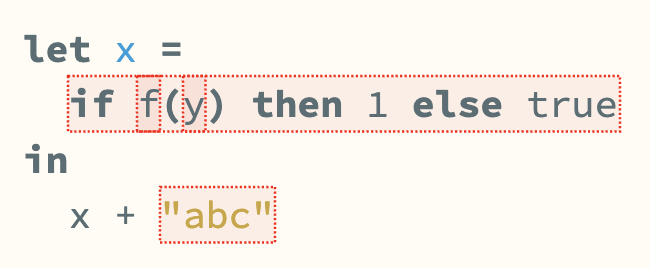
\includegraphics[scale=0.5]{images/hazel-intro-screenshot.png}
\end{center}

A type checker with no support for error localization or recovery---%
as students in an undergraduate course might write---%
would simply report that this program is ill-typed. 
A more practical approach, and one common even in production type checkers, 
is to localize the first error that causes local type inference to fail and emit an explanatory error message.
In this example, the system might report that the variable \li{f} located on Line 2 is unbound, then stop.

A language server with support for type error recovery would 
 be tasked with continuing past this first error.
 The general difficulty here is that there is now missing semantic information, namely the type of \li{f}, that 
 the bidirectional type system as specified 
 would appear to demand in order to proceed, here in order to determine which type the argument, \li{y}, is to be analyzed against.
 Intuitively, however, it seems that this type is actually \emph{unnecessary} to make an error localization decision about \li{y}: 
it is unbound, so a second error can be simultaneously localized despite the missing information.

To recover further, we might choose to also ignore the bidirectional type system's demand that the guard be confirmed to be a boolean expression 
(because the type of \li{f(y)} is also not well-defined) 
and continue into its branches, observing that they have inconsistent types, \li{Int} and \li{Bool}. 
There are several ways to localize this error. 
One approach would be to assume, arbitrarily, that one branch is correct, localizing the error to the other branch. 
Heuristics have been developed to help make this choice less arbitrary, e.g. 
by observing recent editing history \todo{cite}, 
or training a machine learning model \todo{cite}. 
The other approach, which Hazel takes, is to localize the inconsistency to the conditional expression itself, reporting that the problem is that the branch types differ, as indicated in
the screenshot in \autoref{fig:hazel-intro}. When the cursor is on the conditional expression, the Hazel type inspector---a status bar that reports typing information, including type error messages, about the term at the cursor \cite{hannah1}---shows the following error:

TODO\todo{tpye inspector}

This localization decision affects how the system recovers as it proceeds into the let body, \li{x + 1}. 
If localization had assumed that the \li{then} branch correct, as for example in the Elm type checker, then \li{x : Bool} and an error should be reported on the left operand (though this error might mislead the programmer if this earlier localization guess was incorrect).
If the \li{else} branch was chosen, then \li{x : Int} and an error would not be reported. 
If the inconsistency is localized to the conditional expression as a whole, as in our language server, then we again confront the problem of missing type information: 
\li{x} does not have a known type,
though it \emph{is} known to be bound. 
There is no definitive type or binding error here, based on the incomplete information available in the typing context, 
so we choose not to report an error in Hazel.

No matter how localization handles the left operand, we would like to be able to recover and 
localize the type inconsistency on the right operand (the \li{+} operator is integer addition in Hazel).

This informal exercise demonstrates that (1) localization choices can vary, particularly with regard to whether they make \emph{ad hoc} guesses about intent;  
(2) when combined with error recovery, localization decisions can influence downstream localization decisions; and 
(3) error recovery mechanisms must be able to reason without complete knowledge about types and binding. We argue that such semantic subtleties call for a rigorous theoretical treatment of the topic.

This paper develops the first comprehensive {type-theoretic formulation} of type error localization and recovery, called the \emph{marked lambda calculus} (Sec.~\ref{sec:actions}).\todo{sec}
We bring together three individually well-studied ideas: (1) bidirectional typing, which specifies how type and binding information flows from 
type annotations to expressions \cite{pierce,BidirTyping}, (2) gradual typing, which offers a principled approach for recovering from missing type information  \cite{GradualTyping,sieksnapl}\todo{siek05?}, and 
(3) non-empty holes, which function as syntactic membranes marking erroneous terms, which the editor can display directly on-screen \cite{HazelnutPOPL}.

The Hazelnut calculus \cite{HazelnutPOPL} previously brought these ideas together, but its account of type error localization and recovery was partial and tied integrally into its structure editor (see Sec.~\ref{sec:calculus-hazel}). 
We resolve these problems to formally establish, with accompanying metatheory mechanized in Agda, that the marked lambda calculus features \emph{total error recovery}: {every} syntactically well-formed program sketch (a program structure with, optionally, empty holes \cite{sketching}) can be marked, i.e. its errors can be localized, such that the resulting program has a well-defined type and binding structure.
As we define the calculus, we consider a number of situations where error localization decisions are subtle, including conditionals and destructuring let with granular type annotations.

This system, scaled up and implemented in Hazel (Sec.~\ref{sec:calculus-hazel}), solves the semantic gap problem: Hazel's semantic services, which include type hints \cite{potter1}, semantic navigation, semantic code completion \cite{potter1,blinn}, contextualized documentation \cite{potter2}, and, because Hazel is able to evaluate programs with empty and non-empty holes due to prior work \cite{HazelnutLive}, even semantic services that require run-time information, like live testing, 
are available at all times and at all cursor locations, as long as the program sketch is syntactically well-formed.

Prior work has separately considered mechanisms for maintaining syntactically well-formed program sketches during development: manual hole insertion (as is featured in Agda \cite{agda}, GHC Haskell \cite{haskell-holes}, Idris \cite{idris-holes}, and other languages), syntax error recovery \cite{error-reovery}, and structure editing \cite{HazelnutPOPL}. 
Hazel has both a textual syntax and a structure editor, which are briefly described in Sec.~\ref{sec:calculus-hazel}.\todo{sec} 
Marking is not integrated with structure editing, as it was in Hazelnut. 
%offering (1) a textual syntax, which allows the programmer to manually insert empty holes as necessary, (2) a text-like structure editor that offers partial syntax error recovery (inserting holes to maintain well-formedness as long as all matching delimiters have been placed) \cite{tylr}, and (3) a term-based structure editor with total syntax error recovery, i.e. a guarantee that every edit maintains syntactic well-formedness \cite{HazelnutPOPL}\todo{popl17}. 
However, as a secondary contribution, 
we briefly discuss in Sec.~\ref{sec:calculus-structured-editing} how (1)  total marking can resolve the problem of undefined editing behavior in the Hazelnut structure editor calculus, 
and (2) integrating marking with typed structure editing allows us to re-mark only where necessary based on the edit location and the type and binding structure.

Local type inference pairs well with type error localization and recovery because information flows systematically through the tree, leading to predictable and systematic localization decisions (as informally observed also by \cite{pierce}). Languages with constraint-based type inference gather constraints from all relevant locations in a program. This approach is powerful, but it is also notorious for complicating type error localization and recovery, because inconsistencies can arise through a confluence of constraints originating from any number of locations in the program. 
Complex techniques, e.g. based on machine learning or manual weighting, have been proposed to heuristically localize these errors to expressions. 
In Sec.~\ref{sec:thi}\todo{sec}, we describe how we blend local and constraint-based type inference in Hazel. In particular,  
we generate constraints for each type hole that appears in the program explicitly or that is  generated internally during the  bidirectional type error localization and recovery process from Sec.~\ref{sec:calculus}. 
We develop a unification algorithm that can recover from inconsistent constraints by maintaining possible type hole fillings. For holes that can be uniquely solved, we suggest the solution. 
If conflicting constraints arise, we localize the errors to the relevant type holes, rather 
than attempting to localize to expressions. 
The user can explore the different partial type hole fillings. Making a choice then allows the bidirectional system to localize the error to relevant expressions.
Until the choice is finalized, the system continues to recover gradually.




let x : ? = ? in 
if x then x(x + 1) else 0


bool int int -> int



if x then >x<(>x< + 1) else 0

if >x< then >x<(x + 1) else 0

if >x< then x(>x< + 1) else 0
